% Created 2022-07-22 Fri 16:55
% Intended LaTeX compiler: pdflatex
\documentclass[presentation,aspectratio=1610]{beamer}
\usepackage[utf8]{inputenc}
\usepackage[T1]{fontenc}
\usepackage{graphicx}
\usepackage{grffile}
\usepackage{longtable}
\usepackage{wrapfig}
\usepackage{rotating}
\usepackage[normalem]{ulem}
\usepackage{amsmath}
\usepackage{textcomp}
\usepackage{amssymb}
\usepackage{capt-of}
\usepackage{hyperref}
\usepackage{pifont}
\newcommand{\cmark}{\textcolor{green!80!black}{\ding{51}}}
\usepackage{amssymb}
\usepackage{pgfplotstable}
\DeclareMathOperator{\shift}{q}
\DeclareMathOperator{\diff}{p}
\usepackage{khpreamble, euscript}
\DeclareMathOperator{\atantwo}{atan2}
\newcommand*{\ctrb}{\EuScript{C}}
\newcommand*{\obsv}{\EuScript{O}}
\usetheme{default}
\author{Kjartan Halvorsen}
\date{\today}
\title{State space models}
\hypersetup{
 pdfauthor={Kjartan Halvorsen},
 pdftitle={State space models},
 pdfkeywords={},
 pdfsubject={},
 pdfcreator={Emacs 26.3 (Org mode 9.4.6)}, 
 pdflang={English}}
\begin{document}

\maketitle



\section{PMSM - sysid}
\label{sec:orga9605c3}

\begin{frame}[label={sec:orgfef55c8}]{Obtain state-space model from discrete-time pulse-transfer function}
\end{frame}

\begin{frame}[label={sec:org19ac69e}]{The permanent magnet synchronous motor}
\begin{center}
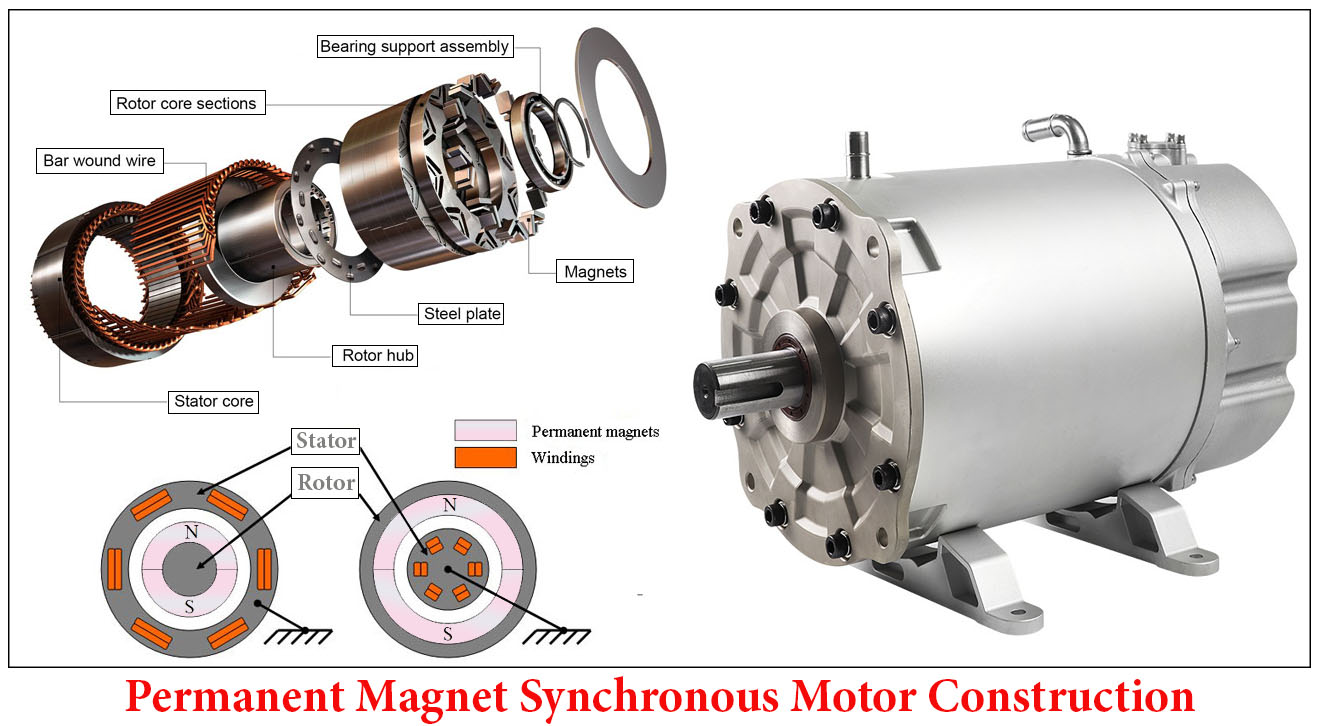
\includegraphics[width=0.9\linewidth]{../../figures/permanent-motor.jpg}
\end{center}
\end{frame}

\begin{frame}[label={sec:org08ae0d8}]{The PMSM}
\begin{center}
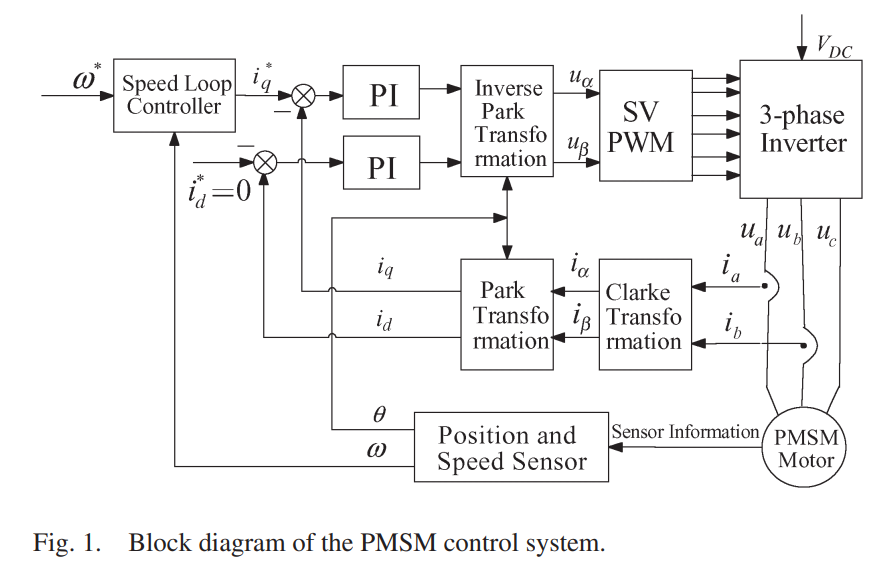
\includegraphics[width=0.8\linewidth]{../../figures/pmsm_control_block_diag.png}
\end{center}
{\footnotesize De Liu and Li  ``Speed control for PMSM servo system'', IEEE Transactions on Industrial Electronics, 2012.}
\end{frame}
\begin{frame}[label={sec:org11978d1}]{Identified model}
Three poles, two zeros
\begin{center}
  \begin{tikzpicture}[node distance=22mm, block/.style={rectangle, draw, minimum width=10mm}, sumnode/.style={circle, draw, inner sep=2pt}]

    % \node[coordinate] (input) {};
    % \node[block, right of=input] (delay1)  {$\frac{1}{z}$};
    % \node[block, right of=delay1, node distance=30mm] (plant)  {$\frac{b_0z^2 + b_1z + b_2}{z^2 + a_1 z + a_2}$};
    % \node[coordinate, right of=plant] (output) {};

    % \draw[->] (input) -- node[above, pos=0.3] {$u(k)$} (delay1);
    % \draw[->] (delay1) -- node[above, pos=0.3] {} (plant);
    % \draw[->] (plant) -- node[above, near end] {$y(k)$} (output);

    % \begin{scope}[yshift=-1cm, xshift = 3cm]
    % \node {$\Updownarrow$};
    % \end{scope}
    % \begin{scope}[yshift=-3cm, xshift = 3cm]
    % \node {$\Updownarrow$};
    % \end{scope}

    % \node[coordinate, below of=input, node distance=2cm] (input2) {};
    % \node[block, right of=input2, node distance=30mm] (plant)  {$\frac{b_0z^2 + b_1z + b_2}{z^2 + a_1 z + a_2}$};
    % \node[block, right of=plant] (delay2)  {$\frac{1}{z}$};
    % \node[coordinate, right of=delay2] (output) {};

    % \draw[->] (input2) -- node[above, pos=0.3] {$u(k)$} (plant);
    % \draw[->] (plant) -- node[above, pos=0.3] {} (delay2);
    % \draw[->] (delay2) -- node[above, near end] {$y(k)$} (output);

    \node[coordinate, below of=input2, node distance=2cm] (input3) {};
    \node[block, right of=input3, node distance=30mm] (plant)  {$\frac{b_0z^2 + b_1z + b_2}{z^3 + a_1 z^2 + a_2z + a_3})$};
    \node[coordinate, right of=plant, node distance=30mm] (output) {};

    \draw[->] (input3) -- node[above, pos=0.3] {$u(k)$} (plant);
    \draw[->] (plant) -- node[above, near end] {$y(k)$} (output);



  \end{tikzpicture}
\end{center}
\end{frame}

\begin{frame}[label={sec:orgf700ceb}]{Identified model}
\[ H(z) = \frac{4.6z^2 + 20.0z -1.0}{z^3 - 1.25z^2 + 0.42z - 0.16}\]

\begin{center}
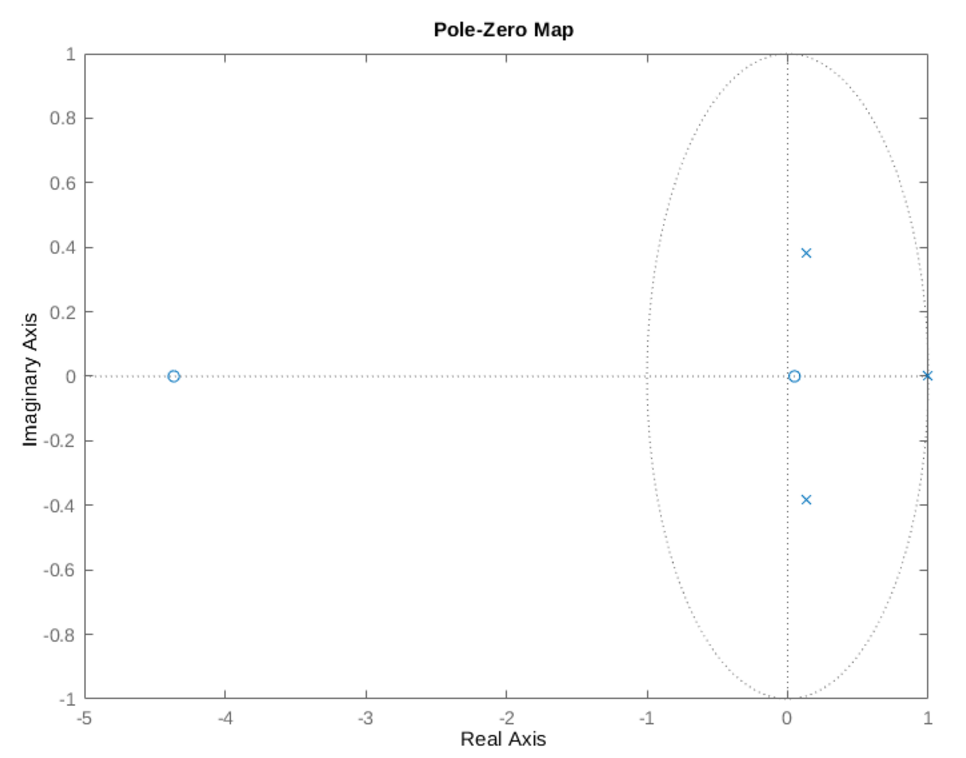
\includegraphics[width=0.45\linewidth]{../../figures/pmsm_arx331_pzmap.png}
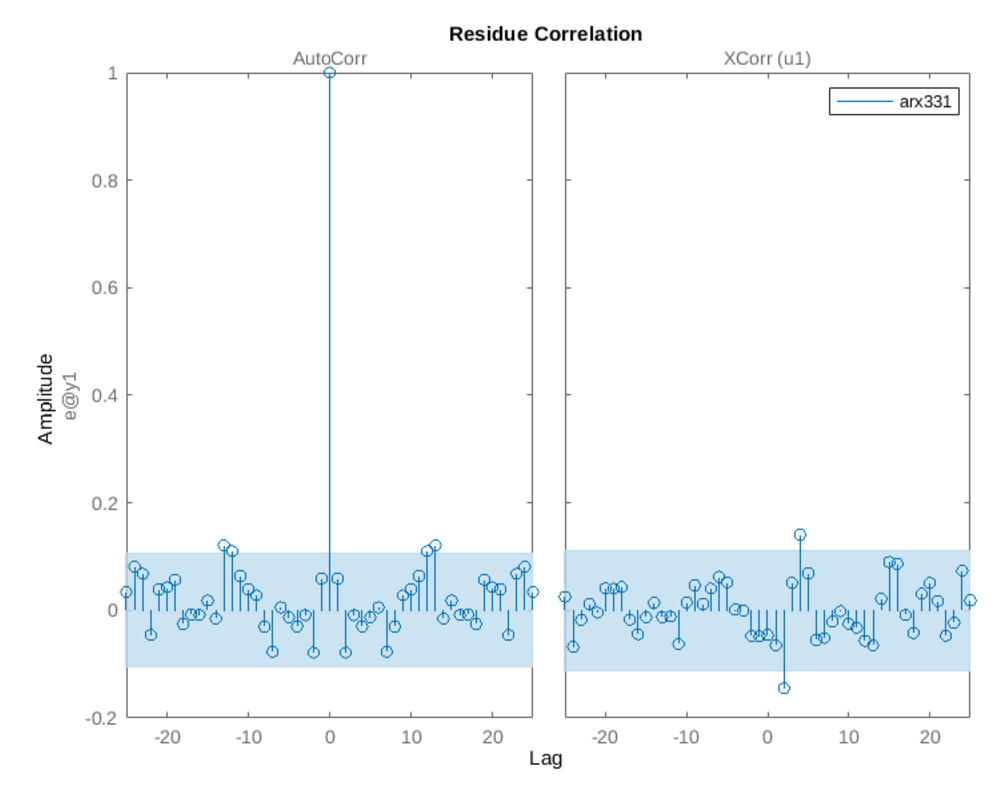
\includegraphics[width=0.45\linewidth]{../../figures/pmsm_arx331_residual.png}
\end{center}
\end{frame}

\begin{frame}[label={sec:orge251605}]{From pulse-transfer function to state space model}
\begin{center}
  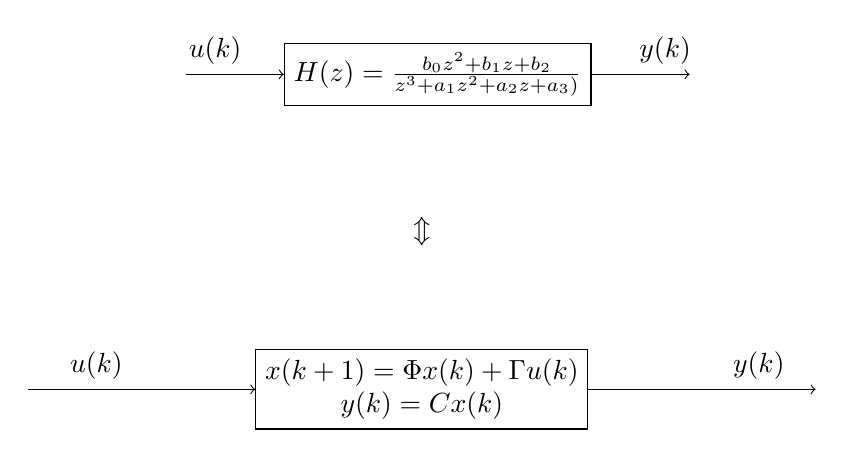
\begin{tikzpicture}[node distance=32mm, block/.style={rectangle, draw, minimum width=15mm}, sumnode/.style={circle, draw, inner sep=2pt}]

    \node[coordinate] (input) {};
    \node[block, right of=input] (plant)  {$H(z) = \frac{b_0z^2 + b_1z + b_2}{z^3 + a_1 z^2 + a_2z + a_3)}$};
    \node[coordinate, right of=plant] (output) {};

    \draw[->] (input) -- node[above, pos=0.3] {$u(k)$} (plant);
    \draw[->] (plant) -- node[above, near end] {$y(k)$} (output);

    \begin{scope}[yshift=-2cm, xshift = 3cm]
    \node {$\Updownarrow$};
    \end{scope}

    \begin{scope}[yshift=-4cm, node distance=50mm, xshift=-2cm]
    \node[coordinate] (input) {};
    \node[block, right of=input, align=center] (plant)  {$x(k+1) = \Phi x(k) + \Gamma u(k)$\\$y(k) = C x(k)$};
    \node[coordinate, right of=plant] (output) {};

    \draw[->] (input) -- node[above, pos=0.3] {$u(k)$} (plant);
    \draw[->] (plant) -- node[above, near end] {$y(k)$} (output);
    \end{scope}



  \end{tikzpicture}
\end{center}
\end{frame}

\begin{frame}[label={sec:org51c8988}]{Canonical forms}
Given pulse-transfer function 
\[ H(z) = \frac{b_1 z^2 + b_2 z + b_3}{z^3 + a_1z^2 + a_2z + a_3}.\] 
Find a representation in state space form
\begin{align*}
 x(k+1) &= \Phi x(k) + \Gamma u(k) \\
 y(k) &= C x(k)
 \end{align*}

\pause

\begin{itemize}
\item Controlable canonical form
\item Observable canonical form
\end{itemize}
\end{frame}

\begin{frame}[label={sec:org7513c03}]{Controlable canonical form}
Given pulse-transfer function 
\[ H(z) = \frac{b_1 z^2 + b_2 z + b_3}{z^3 + a_1z^2 + a_2z + a_3}.\] 

\begin{align*}
 x(k+1) &= \begin{bmatrix} -a_1 & -a_2 & -a_3\\1 & 0 & 0\\0 & 1 & 0\end{bmatrix} x(k) + \begin{bmatrix}1\\0\\0\end{bmatrix} u(k) \\
 y(k) &= \begin{bmatrix} b_1 & b_2 & b_3 \end{bmatrix} x(k)
 \end{align*}
\end{frame}


\begin{frame}[label={sec:org2bef48e}]{Observable canonical form}
Given pulse-transfer function 
\[ H(z) = \frac{b_1 z^2 + b_2 z + b_3}{z^3 + a_1z^2 + a_2z + a_3}.\] 

\begin{align*}
 x(k+1) &= \begin{bmatrix} -a_1 & 1 & 0\\-a_2 & 0 & 1\\-a_3 & 0 & 0\end{bmatrix} x(k) + \begin{bmatrix}b_1\\b_2\\b_3\end{bmatrix} u(k) \\
 y(k) &= \begin{bmatrix} 1 & 0 & 0 \end{bmatrix} x(k)
 \end{align*}
\end{frame}


\begin{frame}[label={sec:org982ed49}]{Canonical forms}
\alert{Activity} Find the controlable and observable canonical forms for the pulse-transfer function of the motor. Answer on Canvas (questions 1 and 2 on today's exercises).

\[ H(z) = \frac{4.6z^2 + 20.0z -1.0}{z^3 - 1.25z^2 + 0.42z - 0.16}\]
\end{frame}


\section{Apollo moon lander}
\label{sec:orgcf9afff}
\begin{frame}[label={sec:orgde33206}]{Discrete-time state-space  from continuous-time state space}
A.k.a. discretization
\end{frame}

\begin{frame}[label={sec:org884f995}]{Example - the Apollo lunar module}
\begin{center}
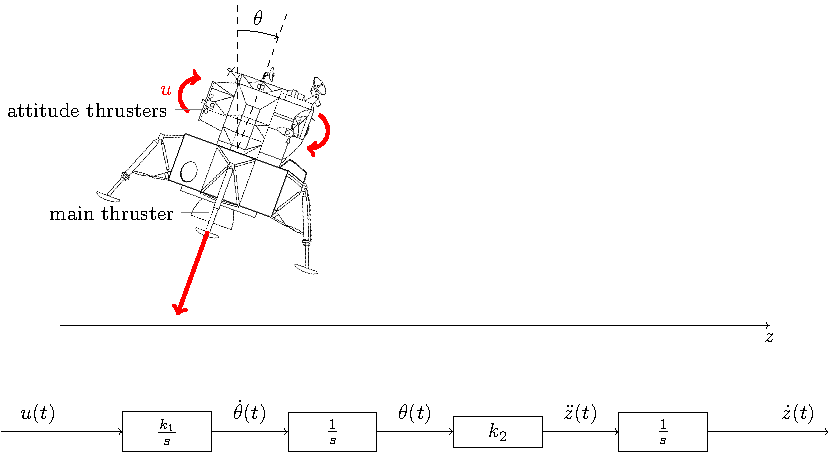
\includegraphics[width=\linewidth]{fig-apollo}
\end{center}
\end{frame}
\begin{frame}[label={sec:org88a3e4a}]{Example - the Apollo lunar module}
\begin{center}
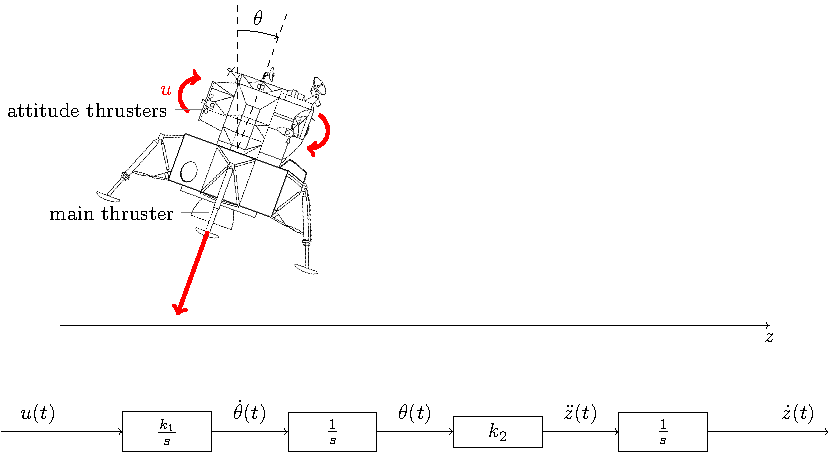
\includegraphics[width=0.8\linewidth]{fig-apollo}
\end{center}
\alert{Activity} Which is the transfer function of the system?
\[1: \; G(s) = \frac{k_1 k_2}{s^2}\qquad 2: \; G(s) = \frac{k_1 k_2}{s(s^2 + 1)} \qquad 3: \; G(s) = \frac{k_1 k_2}{s^3}\]
\end{frame}

\begin{frame}[label={sec:orgedc44d8}]{Example - the Apollo lunar module}
\begin{center}
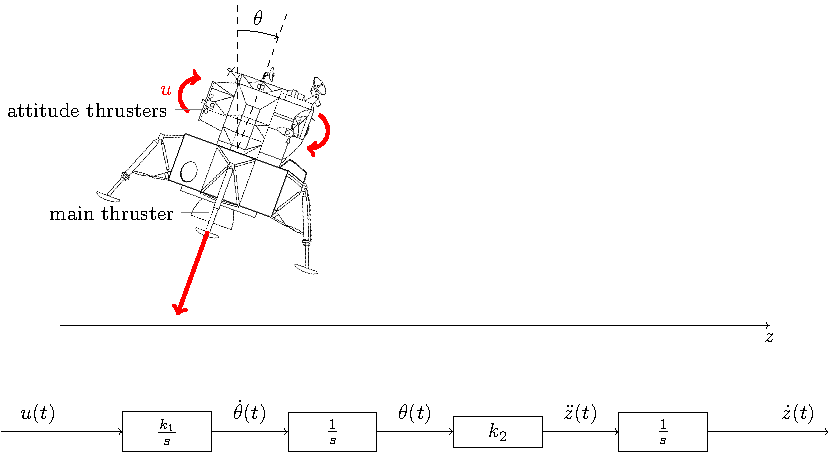
\includegraphics[width=0.8\linewidth]{fig-apollo}
\end{center}
\alert{Activity} What sensors are needed by the control system?
\end{frame}

\begin{frame}[label={sec:org09e1bba}]{Example - the Apollo lunar module}
\begin{center}
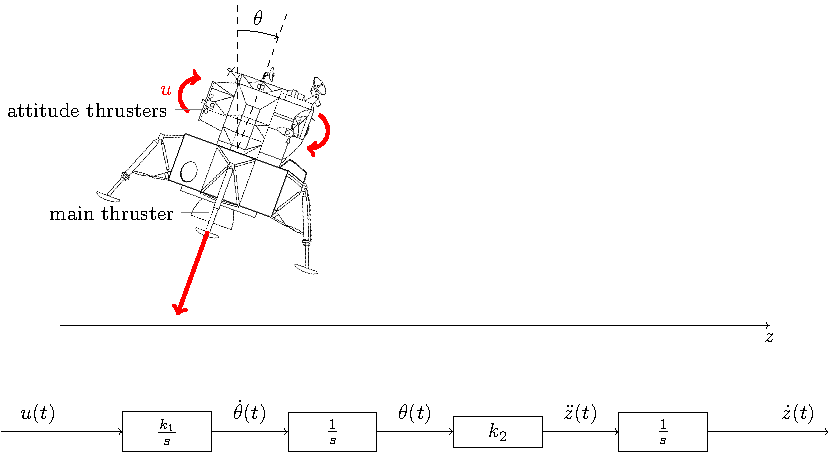
\includegraphics[width=0.7\linewidth]{fig-apollo}
\end{center}

State variables: \(x = \begin{bmatrix} x_1 & x_2 & x_3 \end{bmatrix}^T = \begin{bmatrix} \dot{\theta} & \theta & \dot{z} \end{bmatrix}^T\). With the dynamics
\[ \begin{cases} \dot{x}_1 =  \ddot{\theta} = k_1 u\\ \dot{x}_2 = \dot{\theta} = x_1\\ \dot{x}_3 = \ddot{z} = k_2\theta = k_2x_2 \end{cases} \]
\end{frame}

\begin{frame}[label={sec:orgc66d921}]{Example - the Apollo lunar module}
State variables: \(x = \begin{bmatrix} x_1 & x_2 & x_3 \end{bmatrix}^T = \begin{bmatrix} \dot{\theta} & \theta & \dot{z} \end{bmatrix}^T\). With dynamics
\[ \begin{cases} \dot{x}_1 =  \ddot{\theta} = k_1 u\\ \dot{x}_2 = \dot{\theta} = x_1\\ \dot{x}_3 = \ddot{z} = k_2\theta = k_2x_2 \end{cases} \]

\alert{Activity} Fill the matrix \(A\) and vector \(B\).

\[ \dot{x} = \begin{bmatrix} \dot{x}_1\\\dot{x}_2\\\dot{x}_3\end{bmatrix} = \underbrace{\begin{bmatrix} \textcolor{white}{0} & \textcolor{white}{0} &\textcolor{white}{0} \\\textcolor{white}{1} & \textcolor{white}{0}& \textcolor{white}{0}\\ \textcolor{white}{0}& \textcolor{white}{k_2} &\textcolor{white}{0} \end{bmatrix}}_{A} \begin{bmatrix} x_1\\x_2\\x_3\end{bmatrix} + \underbrace{\begin{bmatrix} \textcolor{white}{k_1} \\ \textcolor{white}{0} \\\textcolor{white}{0}  \end{bmatrix}}_{B} u \]
\end{frame}

\begin{frame}[label={sec:org1f8222f}]{Example - the Apollo lunar module}
\end{frame}


\section{Discretization}
\label{sec:org5295fa1}

\begin{frame}[label={sec:org5cb34e5}]{Discretizing a continuous-time state-space model}
\end{frame}
\begin{frame}[label={sec:org405ee0b}]{Discretización}
The general solution to a linear, continuous-time state-space system
\begin{align*}
x(t_k+\tau)& = \mathrm{e}^{A\tau} x(t_k) + \int_{0}^\tau \mathrm{e}^{As} B u\big((t_k+\tau)-s) ds
\end{align*}

\begin{center}
  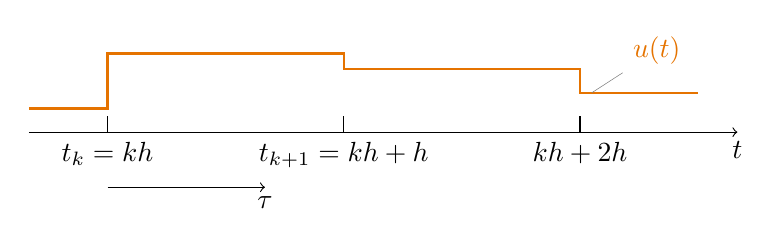
\begin{tikzpicture}
    \draw[->] (-3,0) -- (6,0) node[below] {$t$};
    \draw (-2, 0.2) -- ( -2, 0) node[below] {$t_k=kh$};
    \draw (1, 0.2) -- ( 1, 0) node[below] {$t_{k+1}=kh+h$};
    \draw (4, 0.2) -- ( 4, 0) node[below] {$kh+2h$};
    \draw[thick, orange!90!black] (-3,0.3) -- (-2, 0.3) -- (-2,1) -- (1, 1) -- (1,0.8) -- (4, 0.8) --(4, 0.5) --(5.5, 0.5) node[pos=0.1, coordinate, pin=30:{$u(t)$}] {} ; 
    \draw[->] (-2, -0.7) -- (0, -0.7) node[below] {$\tau$};
  \end{tikzpicture}
\end{center}

 \begin{align*}
  x(kh+h) &= \mathrm{e}^{Ah} x(kh) + \int_{0}^{h} \mathrm{e}^{As} B u(kh+h-s) ds\\
   &= \underbrace{\mathrm{e}^{Ah}}_{\Phi(h)} x(kh) + \underbrace{\left(\int_{0}^h \mathrm{e}^{As} B ds \right)}_{\Gamma(h)} u(kh)
\end{align*}
\end{frame}

\begin{frame}[label={sec:org94d39e8}]{Discretization - The matrix exponential}
Square matrix \(A\). Scalar variable \(t\).
\[ \mathrm{e}^{At} = I + At + \frac{t^2}{2!}A^2 + \frac{t^3}{3!} A^3 + \cdots\]
Laplace transform
\[ \laplace{\mathrm{e}^{At}} = (sI - A)^{-1}\]
\end{frame}


\begin{frame}[label={sec:org8b97ae2}]{Discretization - example}
 \begin{align*}
  x(kh+h) &= \mathrm{e}^{Ah} x(kh) + \int_{0}^{h} \mathrm{e}^{As} B u(kh+h-s) ds\\
   &= \underbrace{\mathrm{e}^{Ah}}_{\Phi(h)} x(kh) + \underbrace{\left(\int_{0}^h \mathrm{e}^{As} B ds \right)}_{\Gamma(h)} u(kh)
\end{align*}
\[ A = \begin{bmatrix} 0 & 0 & 0\\1 & 0 & 0\\0 & k_2 & 0\end{bmatrix}, \quad A^2 = \begin{bmatrix} 0 & 0 & 0\\1 & 0 & 0\\0 & k_2 & 0\end{bmatrix}\begin{bmatrix} 0 & 0 & 0\\1 & 0 & 0\\0 & k_2 & 0\end{bmatrix}= \begin{bmatrix} 0 & 0 & 0\\0 & 0 & 0\\k_2 & 0  & 0\end{bmatrix}, \quad A^3 = 0\]
So,
\begin{align*}
 \Phi(h) &= \mathrm{e}^{Ah} = 1 + Ah + A^2 h^2/2  + \cdots \\
 &= \begin{bmatrix} 1 & 0 & 0\\0 & 1 & 0\\0 & 0 & 1\end{bmatrix} + \begin{bmatrix} 0 & 0 & 0\\1 & 0 & 0\\0 & k_2 & 0\end{bmatrix}h + \begin{bmatrix} 0 & 0 & 0\\0 & 0 & 0\\k_2 & 0 & 0\end{bmatrix}\frac{h^ 2}{2}= \begin{bmatrix} 1 & 0 & 0\\h & 1 & 0\\\frac{h^2k_2}{2} & hk_2 & 1\end{bmatrix}
 \end{align*}
\end{frame}

\begin{frame}[label={sec:orgad0931e}]{Discretization - example}
 \begin{align*}
  x(kh+h) &= \mathrm{e}^{Ah} x(kh) + \int_{0}^{h} \mathrm{e}^{As} B u(kh+h-s) ds\\
   &= \underbrace{\mathrm{e}^{Ah}}_{\Phi(h)} x(kh) + \underbrace{\left(\int_{0}^h \mathrm{e}^{As} B ds \right)}_{\Gamma(h)} u(kh)
\end{align*}
\[\mathrm{e}^{As}B &=  \begin{bmatrix} 1 & 0 & 0\\s & 1 & 0\\\frac{s^2k_2}{2} & sk_2 & 1\end{bmatrix} \begin{bmatrix} k_1\\0\\0 \end{bmatrix} = k_1 \begin{bmatrix} 1\\s\\\frac{k_2s^2}{2} \end{bmatrix}
  \]
\begin{align*}
\Gamma (h) &= \int_0^h \mathrm{e}^{As}B ds = k_1 \int_0^h \begin{bmatrix} 1\\s\\\frac{k_2s^2}{2} \end{bmatrix}ds = k_1\begin{bmatrix} h\\ \frac{h^2}{2} \\ \frac{k_2 h^3}{6} \end{bmatrix} 
\end{align*}
\end{frame}

\begin{frame}[label={sec:org7ceede2}]{Discretization - example}
 \begin{align*}
  x(kh+h) &= \mathrm{e}^{Ah} x(kh) + \int_{0}^{h} \mathrm{e}^{As} B u(kh+h-s) ds\\
   &= \underbrace{\mathrm{e}^{Ah}}_{\Phi(h)} x(kh) + \underbrace{\left(\int_{0}^h \mathrm{e}^{As} B ds \right)}_{\Gamma(h)} u(kh)\\
   &= \begin{bmatrix} 1 & 0 & 0\\h & 1 & 0\\\frac{h^2k_2}{2} & hk_2 & 1\end{bmatrix} x(kh) + k_1 \begin{bmatrix} h\\ \frac{h^2}{2} \\ \frac{k_2 h^3}{6} \end{bmatrix} u(kh)
\end{align*}
\end{frame}

\begin{frame}[label={sec:orgec19f3f}]{Discretization - exercise}
\alert{Activity} Discretize the system (question 3 on today's exercises on Canvas)
\[ \dot{x} = Ax + Bu = \begin{bmatrix} 0 & 1\\ 0 & 0 \end{bmatrix} x + \begin{bmatrix}0\\1\end{bmatrix}u\]
\end{frame}
\end{document}